\section{Multi-class Logistic Regression}

One way to extend logistic regression to multi-class (say $K$ class labels) setting is to consider $(K-1)$ sets of weight vectors and define
\[
P(Y = y_k \mid X) = \frac{\exp \left( w_{k0} + \sum_{i=1}^d w_{ki}x_i \right)}{\sum_{j=1}^{K-1} \exp \left( w_{j0} + \sum_{i=1}^d w_{ji}x_i \right)}, \quad \text{for } k = 1, \ldots, K-1
\]

\subsection{part 1}

What does this model imply for $P(Y = y_k \mid X)$?
\begin{qsolve}
	\begin{qsolve}[]
		$$
		P(Y = y_k \mid X) = 1 - \sum_{k=1}^{K-1} P(Y = y_k \mid X) = 1 - \sum_{k=1}^{K-1} \alpha \exp \left( w_{k0} + \sum_{i=1}^d w_{ki}x_i \right)
		$$
		$$
		\Rightarrow \alpha = \frac{1}{1 + \sum_{k=1}^{K-1} \exp \left( w_{k0} + \sum_{i=1}^d w_{ki}x_i \right)}
		$$
		so the model implies that the probability of the $K$th class is the complement of the sum of the probabilities of the other classes means that:
		\begin{center}
			\hl{$P(Y = y_K \mid X) = \alpha \exp \left( w_{K0} + \sum_{i=1}^d w_{Ki}x_i \right) , \quad \text{for } k = 1,2, \ldots, K-1$}
			\\
			\hl{$P(Y = y_K \mid X) = \alpha,\quad \text{ for } k = K$}
		\end{center}
		
		
	\end{qsolve}
\end{qsolve}
\subsection{part 2}

What would be the classification rule in this case?

\begin{qsolve}
	\begin{qsolve}[]
		the classification rule in this case is to choose the class with the highest probability. for example for class j we choose the class with the highest $P(Y=y_j\mid x)$
	\end{qsolve}
\end{qsolve}

\subsection{part 3}

Draw a set of training data with three labels and the decision boundary resulting from a multi-class logistic regression
The boundary does not need to be quantitatively correct but should qualitatively depict how a typical boundary from multi-class logistic regression would look like.

\begin{qsolve}
	\begin{qsolve}[]
		\begin{figure}[H]
			\centering
			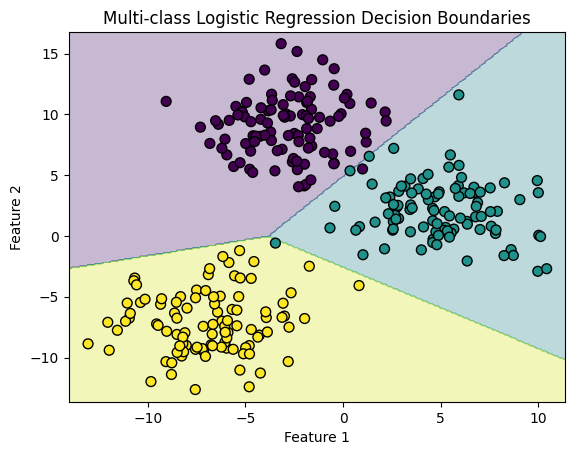
\includegraphics[width=0.7\textwidth]{multi.png}
			\caption{Multi-class logistic regression decision boundary}
		\end{figure}
	\end{qsolve}
\end{qsolve}

\subsection{part 4}

Find log-likelihood if $N$ data sample: $X = \{(x_i, y_i)\}_{i = 1}^N$ is observed

\begin{qsolve}
	\begin{qsolve}[]
		as we proved in part 1 the probability of the $K$th class is:
		$$
		P(Y = y_K \mid X) = \alpha \exp \left( w_{K0} + \sum_{i=1}^d w_{Ki}x_i \right) , \quad \text{for } k = 1,2, \ldots, K-1
		$$
		$$
		P(Y = y_K \mid X) = \alpha,\quad \text{ for } k = K
		$$
		wich $\alpha$ is:
		$$
		\alpha = \frac{1}{1 + \sum_{k=1}^{K-1} \exp \left( w_{k0} + \sum_{i=1}^d w_{ki}x_i \right)}
		$$
		so the log-likelihood of the data is:
		$$
		\mathcal{L}(w) = \sum_{i=1}^{N} \log P(y_i \mid x_i; w)
		$$
		$$
		= \sum_{i=1}^{N} \log \left( \frac{\exp \left( w_{y_i0} + \sum_{j=1}^d w_{y_ij}x_{ij} \right)}{\sum_{k=1}^{K-1} \exp \left( w_{k0} + \sum_{j=1}^d w_{kj}x_{ij} \right)} \right)
		$$
	\end{qsolve}
\end{qsolve}

\subsection{part 5}

Now suppose that we add a L2 regularizing term to this objective function:
\[
f(X) = \log(P(Y \mid X)) - \lambda \sum_{k=1}^K \|w_k\|^2
\]
Now Calculate the gradient of the function $f(X)$ with respect to $w$.
\begin{qsolve}
	\begin{qsolve}[]
		$$
		f(W) = \mathcal{L}(w) - \lambda \sum_{k=1}^K \|w_k\|^2
		$$
		$$
		\Rightarrow \nabla f(W) = \nabla \mathcal{L}(w) - \lambda \nabla \sum_{k=1}^K \|w_k\|^2
		$$
		$$
		= \nabla \mathcal{L}(w) - 2\lambda w
		$$
		$$
		\Rightarrow \nabla_{w} f(W) = \sum_{i=1}^{N} \left[ \frac{x_i \exp(w_k^T x_i)}{1 + \sum_{j=1}^{K-1} \exp(w_j^T x_i)} \right] - 2w_k
		$$
	\end{qsolve}
\end{qsolve}

\subsubsection{part 6}
Write update rule for the dataset $X$ according to the answer of the previous part and simplify as much as possible and explain what happens to $w$ at each iteration
\begin{qsolve}
	\begin{qsolve}[]
		by gradient descent we have:
		$$
		w_{k}^{(t+1)} = w_{k}^{(t)} - \eta \nabla_{w} f(W)
		$$
		$$
		= w_{k}^{(t)} - \eta \left[ \sum_{i=1}^{N} \left[ \frac{x_i \exp(w_k^{(t)^T} x_i)}{1 + \sum_{j=1}^{K-1} \exp(w_j^{(t)^T} x_i)} \right] - 2w_k^{(t)} \right]
		$$
		
	\end{qsolve}
\end{qsolve}
